\documentclass{article}
\usepackage[utf8]{inputenc}
\usepackage{amsmath}
\usepackage{amssymb}
\usepackage[makeroom]{cancel}
\usepackage{tabularx}
\usepackage{graphicx}

\setlength{\parskip}{1em}
\setlength\parindent{0px}
\title{Homework 2}
\date{\today}
\author{John J Li}

\begin{document}
    \pagenumbering{gobble}
    \maketitle
    \newpage
    \pagenumbering{arabic}

    \textbf{Problem 1:}

    \begin{center}
        \begin{tabularx} {\textwidth} {
            >{\raggedright\arraybackslash}X
            >{\raggedright\arraybackslash}X }
    
            $(abc') + (bd) + (a'cd') + (b'd) + (a'c'd')$ & \emph{(1)} \\
            $(bd+b'd) + (a'cd'+a'c'd') + (abc')$ & \emph{(2)} Associative \\
            $d(b+b') + a'd'(c+c') + (abc')$ & \emph{(3)} Distributive \\
            $d\cancel{(b+b')} + a'd'\cancel{(c+c')} + (abc')$ & \emph{(4)} Inverse element \\
            $d + a'd' + abc'$ & \emph{(5)} Identity \\
            $(d+a')(d+d') + abc'$ & \emph{(6)} Distributive \\
            $(d+a')\cancel{(d+d')} + abc'$ & \emph{(7)} Inverse element \\
            $(d+a') + abc'$ & \emph{(8)} Identity \\
            $d + (a'+a)(a'+b)(a'+c')$ & \emph{(9)} Distributive \\
            $d + \cancel{(a'+a)}(a'+b)(a'+c')$ & \emph{(10)} Inverse element \\
            $d + (a'+b)(a'+c')$ & \emph{(11)} Identity \\
            $d + a'+(bc')$ & \emph{(12)} Distributive \\
    
        \end{tabularx}
    \end{center}

    %###################################################################################

    \textbf{Problem 2:}

    \begin{center}
        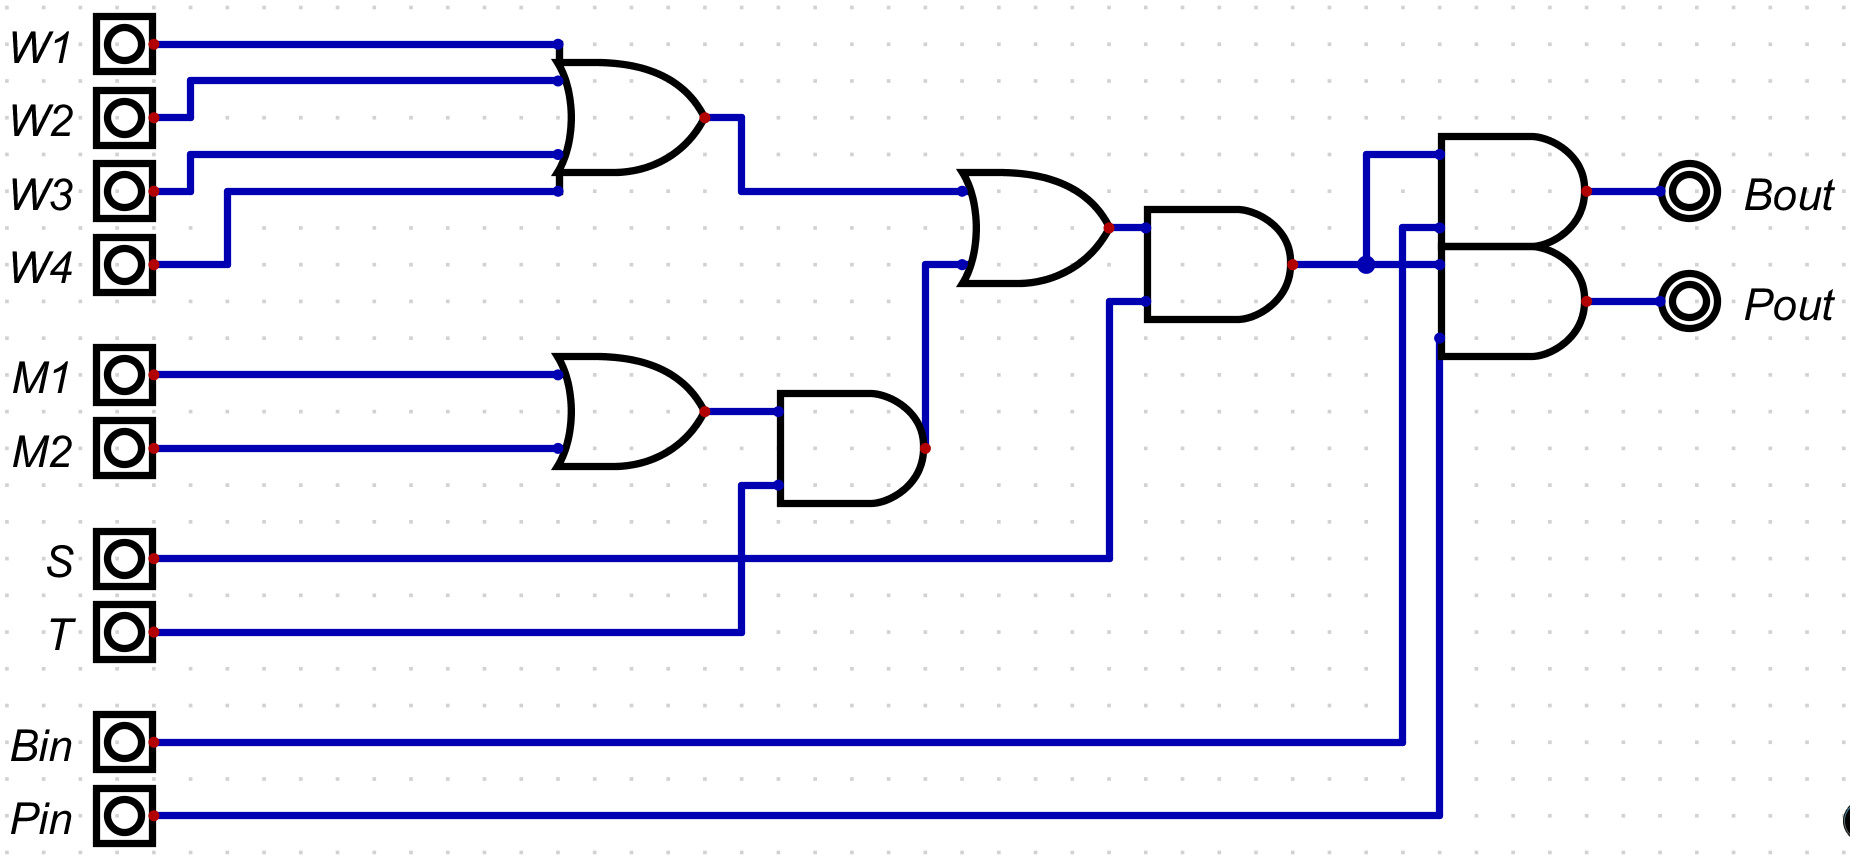
\includegraphics[width=\linewidth]{q2.jpg}
    \end{center}

    %###################################################################################

    \textbf{Problem 3:}

    \quad (a)

    \begin{center}
        \begin{tabular} {cccc|c} 
            \# & x & y & z & G(x,y,z) \\
            \hline
            0 & 0 & 0 & 0 & 1 \\
            1 & 0 & 0 & 1 & 1 \\
            2 & 0 & 1 & 0 & 0 \\
            3 & 0 & 1 & 1 & 1 \\
            4 & 1 & 0 & 0 & 1 \\
            5 & 1 & 0 & 1 & 0 \\
            6 & 1 & 1 & 0 & 0 \\
            7 & 1 & 1 & 1 & 1 \\
        \end{tabular}
    \end{center}

    \quad (b)

    \quad\quad cononical SOP

    \begin{equation*}
        G(x,y,z) = x'y'z' + x'y'z + x'yz + xy'z' + xyz
    \end{equation*}

    \quad (c)

    \begin{center}
        \begin{tabularx} {1.2\textwidth} {
            >{\raggedright\arraybackslash}X
            >{\raggedright\arraybackslash}X }
    
            $G(x,y,z) = x'y'z' + x'y'z + x'yz + xy'z' + xyz$ & \emph{(1)} \\
            $G(x,y,z) = x'y'z' + x'y'z + x'yz + xyz + xy'z'$ & \emph{(2)} Associative \\
            $G(x,y,z) = x'y'(z'+ z) + (x'+x)yz + xy'z'$ & \emph{(3)} Distributive \\
            $G(x,y,z) = x'y'\cancel{(z'+ z)} + \cancel{(x'+x)}yz + xy'z'$ & \emph{(4)} Inverse element \\
            $G(x,y,z) = x'y' + yz + xy'z'$ & \emph{(5)} Identity \\
            $G(x,y,z) = x'y' + xy'z'+ yz$ & \emph{(6)} Associative \\
            $G(x,y,z) = y'(x' + xz')+ yz$ & \emph{(7)} Distributive \\

    
        \end{tabularx}
    \end{center}

    \quad (d)

    \quad\quad cononical POS

    \begin{equation*}
        G(x,y,z) = (x+y'+z) \cdot (x' + y + z') \cdot (x' + y' + z)
    \end{equation*}

    \quad (e)

    \begin{equation*}
        G(x,y,z) = \pi M(2,5,6)
    \end{equation*}

    \quad (f)

    \begin{center}
        \begin{tabularx} {1.2\textwidth} {
            >{\raggedright\arraybackslash}X
            >{\raggedright\arraybackslash}X }
    
            $G(x,y,z) = (x+y'+z) \cdot (x' + y + z') \cdot (x' + y' + z)$ & \emph{(1)} \\
            $G(x,y,z) = (x' + y + z') \cdot (x+y'+z) \cdot (x' + y' + z)$ & \emph{(2) Associative} \\
            $G(x,y,z) = (x' + y + z') \cdot (y'+z)\cdot (x+x')$ & \emph{(3) Distributive} \\
            $G(x,y,z) = (x' + y + z') \cdot (y'+z)\cdot \cancel{(x+x')}$ & \emph{(4) Inverse element} \\
            $G(x,y,z) = (x' + y + z') \cdot (y'+z)$ & \emph{(5) Identity} \\

    
        \end{tabularx}
    \end{center}

    %###################################################################################

    \textbf{Problem 4:}

    \begin{center}
        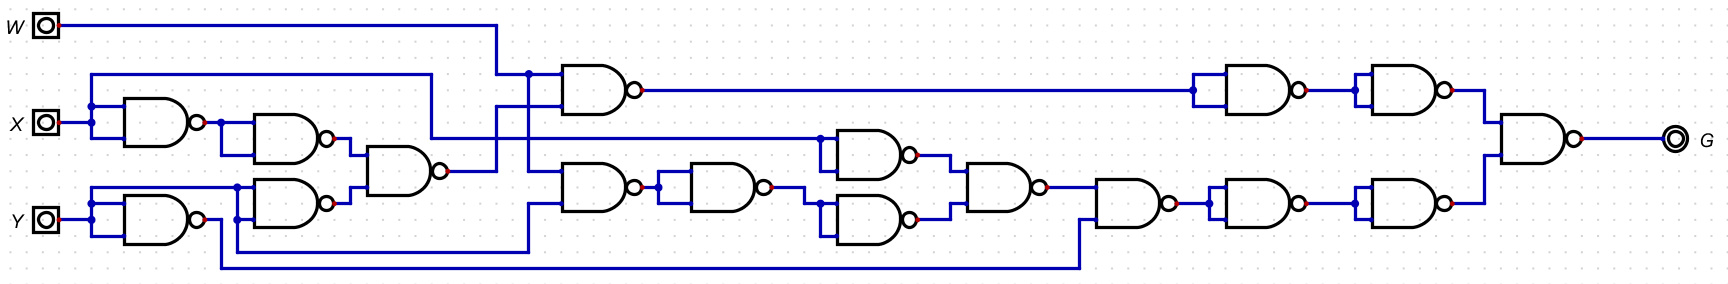
\includegraphics[width=\linewidth]{q4.jpg}
    \end{center}

    \quad\quad Simplified:

    \begin{center}
        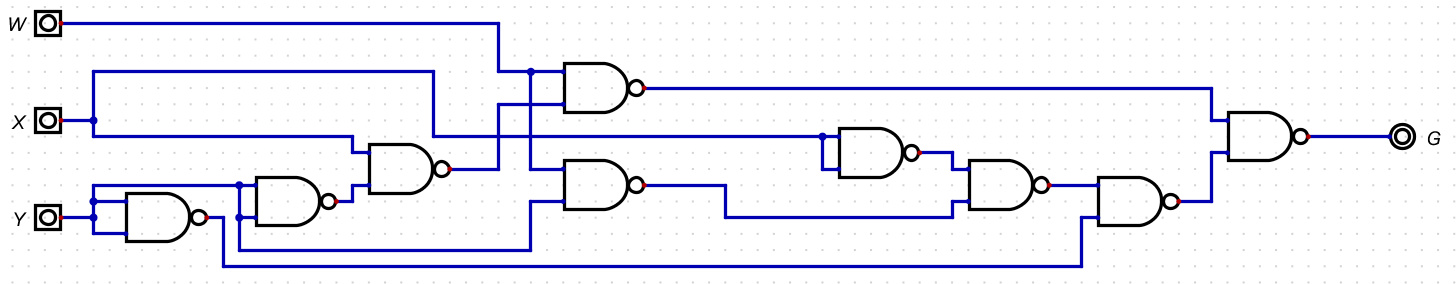
\includegraphics[width=\linewidth]{q4-2.jpg}
    \end{center}

    %###################################################################################

    \textbf{Problem 5:}

    \begin{center}
        \begin{tabular} {ccccccc|c}
            A & B & C & D & A'B'+ABD' & AC'D'+BD' & AB'CD & F \\
            \hline
            0 & 0 & 0 & 0 & 1& 0& 0& 1 \\
            0 & 0 & 0 & 1 & 1& 0& 0& 1 \\
            0 & 0 & 1 & 0 & 1& 0& 0& 1 \\
            0 & 0 & 1 & 1 & 1& 0& 0& 1 \\
            0 & 1 & 0 & 0 & 0& 1& 0& 1 \\
            0 & 1 & 0 & 1 & 0& 0& 0& 0 \\
            0 & 1 & 1 & 0 & 0& 1& 0& 1 \\
            0 & 1 & 1 & 1 & 0& 0& 0& 0 \\
            1 & 0 & 0 & 0 & 0& 1& 0& 1 \\
            1 & 0 & 0 & 1 & 0& 0& 0& 0 \\
            1 & 0 & 1 & 0 & 0& 0& 0& 0 \\
            1 & 0 & 1 & 1 & 0& 0& 1& 1 \\
            1 & 1 & 0 & 0 & 1& 1& 0& 1 \\
            1 & 1 & 0 & 1 & 0& 0& 0& 0 \\
            1 & 1 & 1 & 0 & 1& 1& 0& 1 \\
            1 & 1 & 1 & 1 & 0& 0& 0& 0 \\
        \end{tabular}
    \end{center}

    \begin{center}
        \begin{tabular} {cc|cccc}
            & CD & &&& \\
            AB && 00 & 01 & 11 & 10 \\
            \hline
            & 00 & 1 & 1 & 1 & 1 \\
            & 01 & 1 & 0 & 0 & 1 \\
            & 11 & 1 & 0 & 0 & 1 \\
            & 10 & 1 & 0 & 1 & 0 \\
        \end{tabular}
    \end{center}
    
    0/1/3/2 row: 0000, 0001, 0011, 0010 $\rightarrow$ C and D changes

    \quad $=A'B'$

    0/4/12/8 column: 0000, 0100, 1100, 1000 $\rightarrow$ A and B changes

    \quad $=C'D'$

    3/11 pair: 0011, 1011 $\rightarrow$ A changes

    \quad $=B'CD$

    4/12/6/14 square: 0100, 0110, 1100, 1110 $\rightarrow$ A and C changes

    \quad $=BD'$

    $\boxed{F=A'B'+C'D'+B'CD+BD'}$

    %###################################################################################

    \textbf{Problem 6:}

    \quad (A)

    \begin{center}
        \begin{tabular} {cc|cccc}
            & YZ & &&& \\
            WX && 00 & 01 & 11 & 10 \\
            \hline
            & 00 & 1 & 1 & 0 & 1 \\
            & 01 & 1 & 1 & 0 & 1 \\
            & 11 & 0 & 0 & 0 & 0 \\
            & 10 & 1 & 1 & 0 & 0 \\
        \end{tabular}
    \end{center}

    0/1/4/5/square: 0000, 0001, 0100, 0101 $\rightarrow$ X and Z changes

    \quad $=W'Y'$

    0/1/8/9 square: 0000, 0001, 1000, 1001 $\rightarrow$ W and Z changes

    \quad $=X'Y'$

    0/4/2/6 square: 0000, 0100, 0010, 0110 $\rightarrow$ X and Y changes

    \quad $W'Z'$

    $\boxed{A=W'Y' + X'Y' + W'Z'}$

    \quad (B)

    \begin{center}
        \begin{tabular} {cc|cccc}
            & YZ & &&& \\
            WX && 00 & 01 & 11 & 10 \\
            \hline
            & 00 & 1 & 1 & 1 & 1 \\
            & 01 & 1 & 1 & 1 & 1 \\
            & 11 & 0 & 0 & 0 & 0 \\
            & 10 & 1 & 1 & 1 & 1 \\
        \end{tabular}
    \end{center}

    0/1/3/2/4/5/7/6 rectangle: 0000, 0001, 0011, 0010, 0100, 0101, 0111, 0110
    $\rightarrow$ X, Y, and Z changes

    \quad $=W'$

    0/1/3/2/8/9/11/10 rectangle: 0000, 0001, 0011, 0010, 1000, 1001, 1011, 1010
    $\rightarrow$ W, Y, and Z changes

    \quad $=X'$

    $\boxed{B = W'+X'}$

    %###################################################################################

    \textbf{Problem 7:}

    \begin{center}
        \begin{tabular} {ccccccc|c}
            w & x & y & z & w'y'z & w'xz & yz+xy'z & G \\
            \hline
            0 & 0 & 0 & 0 & 0& 0& 0& 0 \\
            0 & 0 & 0 & 1 & 1& 0& 0& 1 \\
            0 & 0 & 1 & 0 & 0& 0& 0& 0 \\
            0 & 0 & 1 & 1 & 0& 0& 1& 1 \\
            0 & 1 & 0 & 0 & 0& 0& 0& 0 \\
            0 & 1 & 0 & 1 & 1& 1& 1& 1 \\
            0 & 1 & 1 & 0 & 0& 0& 0& 0 \\
            0 & 1 & 1 & 1 & 0& 1& 1& 1 \\
            1 & 0 & 0 & 0 & 0& 0& 0& 0 \\
            1 & 0 & 0 & 1 & 0& 0& 0& 0 \\
            1 & 0 & 1 & 0 & 0& 0& 0& 0 \\
            1 & 0 & 1 & 1 & 0& 0& 1& 1 \\
            1 & 1 & 0 & 0 & 0& 0& 0& 0 \\
            1 & 1 & 0 & 1 & 0& 0& 1& 1 \\
            1 & 1 & 1 & 0 & 0& 0& 0& 0 \\
            1 & 1 & 1 & 1 & 0& 0& 1& 1 \\
        \end{tabular}
    \end{center}

    \begin{center}
        \begin{tabular} {cc|cccc}
            & yz & &&& \\
            wx && 00 & 01 & 11 & 10 \\
            \hline
            & 00 & 0 & 1 & 1 & 0 \\
            & 01 & 0 & 1 & 1 & 0 \\
            & 11 & 0 & 1 & 1 & 0 \\
            & 10 & 0 & 0 & 1 & 0 \\
        \end{tabular}
    \end{center}

    POS

    0/4/12/8/2/6/14/10 rectangle: 0000, 0100, 1100, 1000, 0010, 0110, 1110, 1010
    $\rightarrow$ w,x and y changes

    \quad $=z$

    8/9 pair: 1000, 1001 $\rightarrow$ z changes

    \quad $=w'+x+y$

    $\boxed{G(w,x,y,z) = z(w'+x+y)}$

    SOP

    3/7/15/11 column: 0011, 0111, 1111, 1011 $\rightarrow$ w and x changes

    \quad $=yz$

    5/7/13/15 square: 0101, 0111, 1101, 1111 $\rightarrow$ w and y changes

    \quad $=xz$

    1/3/5/7 square: 0001, 0011, 0101, 0111 $\rightarrow$ x and y changes

    \quad $=w'z$

    $G(w,x,y,z) = yz + xz + w'z$

    %###################################################################################

    \textbf{Problem 8:}

    $F(a,b,c,d) = \sum m (0, 1, 2, 3, 6, 7, 8, 10 ,12, 13)$

    \begin{center}
        \begin{tabular} {cc|cccc}
            & cd & &&& \\
            ab && 00 & 01 & 11 & 10 \\
            \hline
            & 00 & 1 & 1 & 1 & 1 \\
            & 01 & 0 & 0 & 1 & 1 \\
            & 11 & 1 & 1 & 0 & 0 \\
            & 10 & 1 & 0 & 0 & 1 \\
        \end{tabular}
    \end{center}

    0/2/8/10 square: 0000, 0010, 1000, 1010 $\rightarrow$ a and c changed

    \quad $=b'd'$

    0/1/3/2 row: 0000, 0001, 0011, 0010 $\rightarrow$ c and d changed

    \quad $=a'b'$

    3/2/7/6 square: 0011, 0010, 0111, 0110 $\rightarrow$ b and d changed

    \quad $=a'c$

    12/13 pair: 1100, 1101 $\rightarrow$ d changed

    \quad $=abc'$

    $\boxed{F(a,b,c,d) = b'd' + a'b' + a'c + abc'}$

    $G(a,b,c,d) = \sum m (0,1,2,3,8,9,10,13)$

    \begin{center}
        \begin{tabular} {cc|cccc}
            & cd & &&& \\
            ab && 00 & 01 & 11 & 10 \\
            \hline
            & 00 & 1 & 1 & 1 & 1 \\
            & 01 & 0 & 0 & 0 & 0 \\
            & 11 & 0 & 1 & 0 & 0 \\
            & 10 & 1 & 1 & 0 & 1 \\
        \end{tabular}
    \end{center}

    0/2/8/10 square: 0000, 0010, 1000, 1010 $\rightarrow$ a and c changed

    \quad $=b'd'$

    0/1/3/2 row: 0000, 0001, 0011, 0010 $\rightarrow$ c and d changed

    \quad $=a'b'$

    9/13 pair: 1011, 1101 $\rightarrow$ b changed

    \quad $=ac'd$

    $\boxed{G(a,b,c,d) = b'd' + a'b' + ac'd}$

    F Circuit

    \begin{center}
        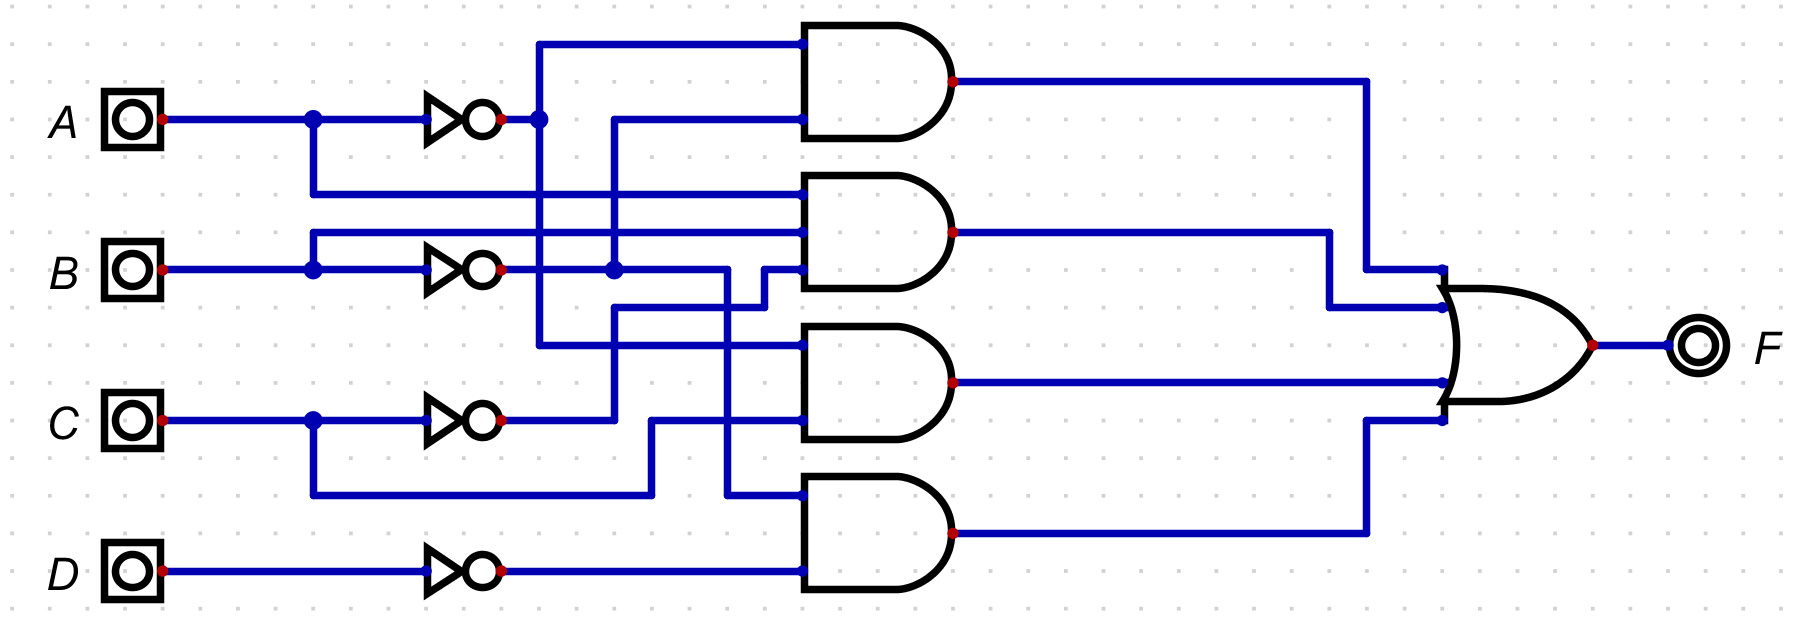
\includegraphics[width=\linewidth]{q8-f.jpg}
    \end{center}

    G Circuit

    \begin{center}
        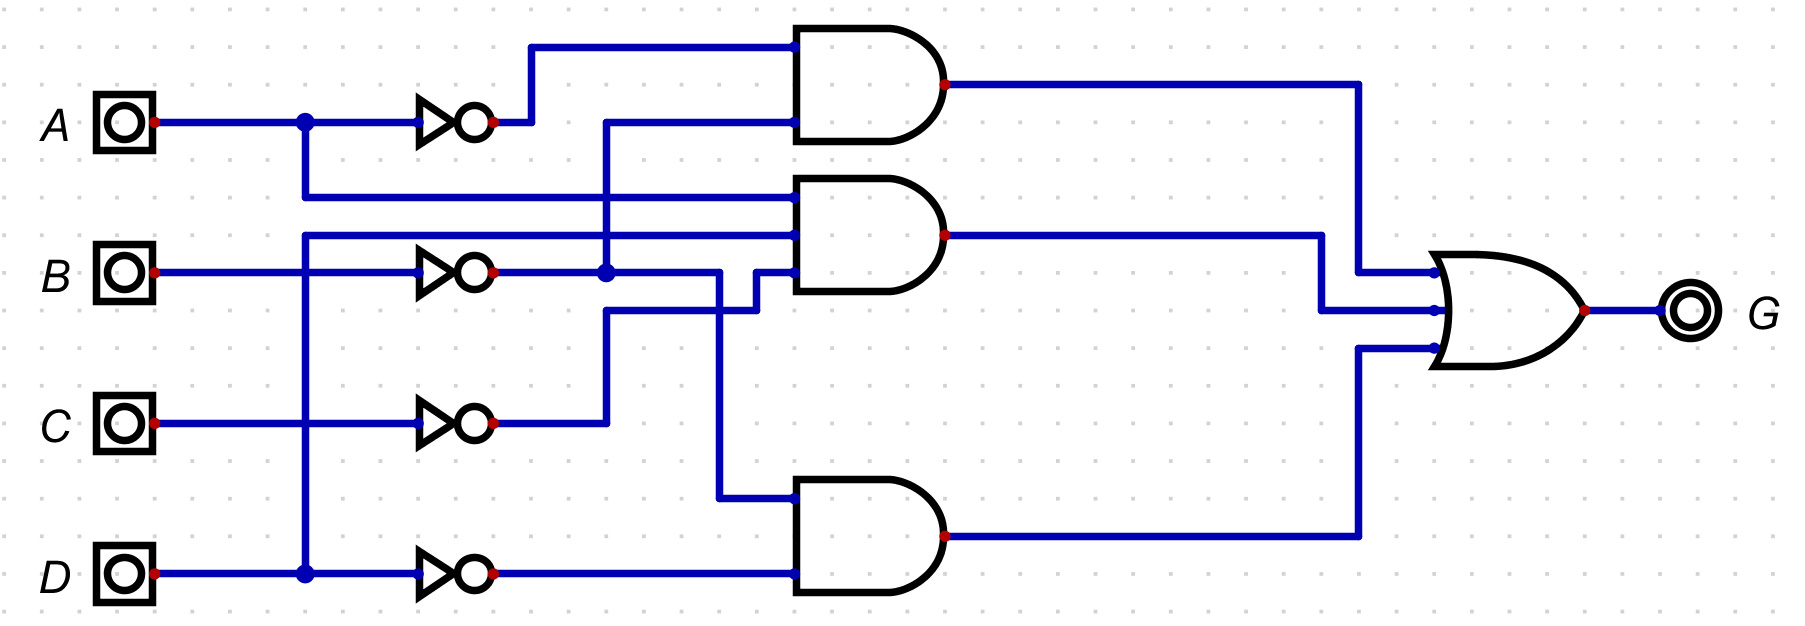
\includegraphics[width=\linewidth]{q8-g.jpg}
    \end{center}

    Shared Circuit

    \begin{center}
        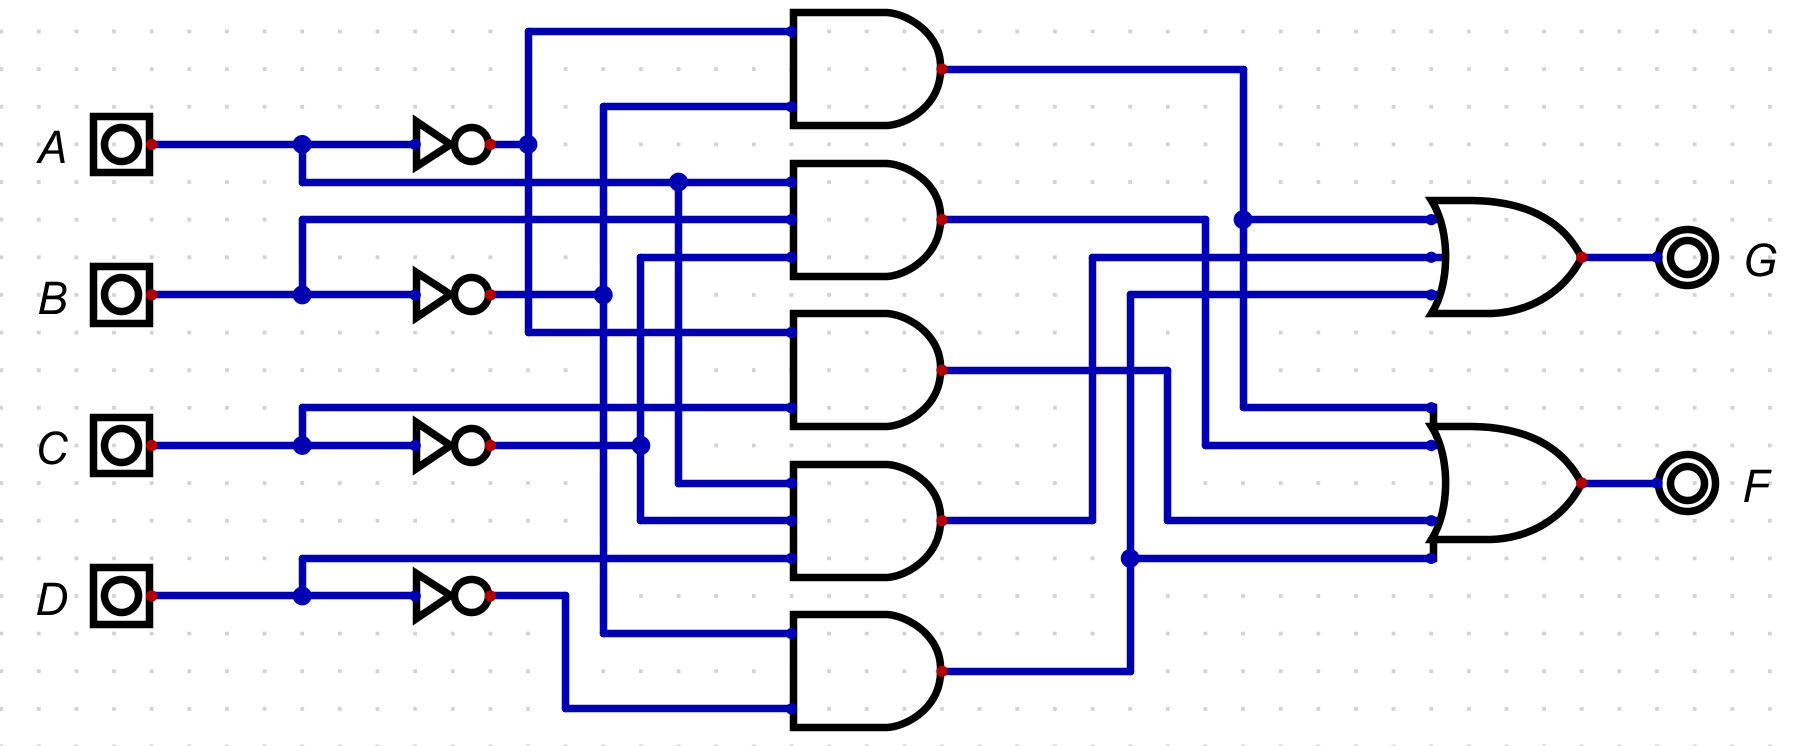
\includegraphics[width=\linewidth]{q8f.jpg}
    \end{center}

    %###################################################################################

    \textbf{Problem 9:}

    $F(a,b,c,d) = \sum m (0,3,4,6,9,10,11,13,14) + \sum d(1,2,7,15)$

    \begin{center}
        \begin{tabular} {cc|cccc}
            & cd & &&& \\
            ab && 00 & 01 & 11 & 10 \\
            \hline
            & 00 & 1 & x & 1 & x \\
            & 01 & 1 & 0 & x & 1 \\
            & 11 & 0 & 1 & x & 1 \\
            & 10 & 0 & 1 & 1 & 1 \\
        \end{tabular}
    \end{center}

    3/2/7/6/15/14/10/11 rectangle: 0011, 0010, 0111, 0110, 1111, 1110, 1011, 1010
    $\rightarrow$ a, b, and d changes

    \quad $=c$

    13/15/9/11 square: 1101, 1111, 1001, 1011 $\rightarrow$ b and c changes

    \quad $=ad$

    0/4/2/6 square: 0000, 0100, 0010, 0110 $\rightarrow$ b and c changes

    \quad $=a'd'$

    $\boxed{c+ad+a'd'}$

    %###################################################################################

    \textbf{Problem 10:}

    \begin{center}
        \begin{tabular} {cccc|c}
            w & x & y & z & G \\
            \hline
            0 & 0 & 0 & 0 & 1 \\
            0 & 0 & 0 & 1 & 0 \\
            0 & 0 & 1 & 0 & 1 \\
            0 & 0 & 1 & 1 & 0 \\
            0 & 1 & 0 & 0 & 1 \\
            0 & 1 & 0 & 1 & 0 \\
            0 & 1 & 1 & 0 & 1 \\
            0 & 1 & 1 & 1 & 0 \\
            1 & 0 & 0 & 0 & 1 \\
            1 & 0 & 0 & 1 & 1 \\
            1 & 0 & 1 & 0 & 1 \\
            1 & 0 & 1 & 1 & 1 \\
            1 & 1 & 0 & 0 & 1 \\
            1 & 1 & 0 & 1 & 1 \\
            1 & 1 & 1 & 0 & 1 \\
            1 & 1 & 1 & 1 & 1 \\
        \end{tabular}
    \end{center}

    \begin{center}
        \begin{tabular} {cc|cccc}
            & yz & &&& \\
            wx && 00 & 01 & 11 & 10 \\
            \hline
            & 00 & 1 & 0 & 0 & 1 \\
            & 01 & 1 & 0 & 0 & 1 \\
            & 11 & 1 & 1 & 1 & 1 \\
            & 10 & 1 & 1 & 1 & 1 \\
        \end{tabular}
    \end{center}

    POS

    1/3/5/7 square: 0001, 0011, 0101, 0111 $\rightarrow$ x and y changes

    \quad $=w+z'$

    $\boxed{G(w,x,y,z) = w+z'}$

    SOP

    1/4/12/8/2/6/14/10 rectangle: 0000, 0100, 1100, 1000, 0010, 0110, 1110, 1010
    $\rightarrow$ w, x, and y changes

    \quad $=z'$

    12/13/15/14/8/9/11/10 rectangle: 1100, 1101, 1111, 1110, 1000, 1001, 1011, 1010
    $\rightarrow$ x, y, and z changes

    \quad $=w$

    $\boxed{G(w,x,y,z) = z' + w}$

\end{document}